\chapter{Implementacja}
% Temporarily change the margins for this page
\newgeometry{
  left=0.5in,
  right=0.5in,
  top=1.5in,
  bottom=1in,
}
\section{Elementy tworzonego systemu}
\begin{figure}[!htbp]
    \centering
    \includesvg[width=\textwidth]{schemas/master-Dev.drawio.svg}
    \caption{Schemat tworzonego systemu}
    \label{fig:enter-label}
\end{figure}

% Restore the original margins
\restoregeometry
\newpage

\begin{figure}[h!]
    \centering
    \begin{msc}[
        title position=center,
        msc keyword=,
        draw frame=none,
        instance distance=2.5cm,
        left environment distance=0.5cm,
        right environment distance=0.5cm,
        label distance=0.3cm,
        title distance=0.5cm
        ]{Protocol Worker Resource Reservation}
            \declinst{user}{}{User}
            \declinst{protocolWorker}{}{Protocol Worker}
            \declinst{serviceDiscovery}{}{Service Discovery}
            \declinst{producer}{}{Producer}
            
            \footnotesize
            \nextlevel
            \mess{Request Resource Reservation}{user}{protocolWorker}
            \nextlevel
            \nextlevel
            \mess{Query All Registered Producers}{protocolWorker}{serviceDiscovery}
            \nextlevel
            \nextlevel
            \nextlevel
            \mess{List of Producers}{serviceDiscovery}{protocolWorker}
            \nextlevel
            \nextlevel
            \nextlevel
            \inlinestart{loop1}{loop for each Producer}{protocolWorker}{producer}
            \nextlevel
            \nextlevel
            \nextlevel
            \nextlevel
            \mess{Check Resource Availability}{protocolWorker}{producer}
            \nextlevel
            \nextlevel
            \nextlevel
            \mess{Resource Availability}{producer}{protocolWorker}
            \nextlevel
            \nextlevel
            \inlineend{loop1}
            \nextlevel
            \nextlevel
            \mess{\parbox{3cm}{Processing producers for products}}{protocolWorker}{protocolWorker}
            \nextlevel
            \nextlevel
            \nextlevel
            \nextlevel
            \nextlevel
            \mess{Return Resource Availability}{protocolWorker}{user}
        \end{msc}
    \caption{ Schemat wymiany wiadomości podczas przetwarzania żądania użytkownika}
    \label{fig:enter-label}
\end{figure}

\subsection{Rejestr usług}

Głównym elementem w podsystemie użytkowym jest rejestr usług, rejestr ten jest wykorzystywany jako zbiór informacji na temat usług uruchomionych w systemie. W usłudze następuje rejestracja producentów świadczący usługi w systemie oraz węzłów protokołu użytkowników, które są wykorzystywane do zarządzania przydziałem zasobów.

\begin{figure}[!htbp]
    \centering
    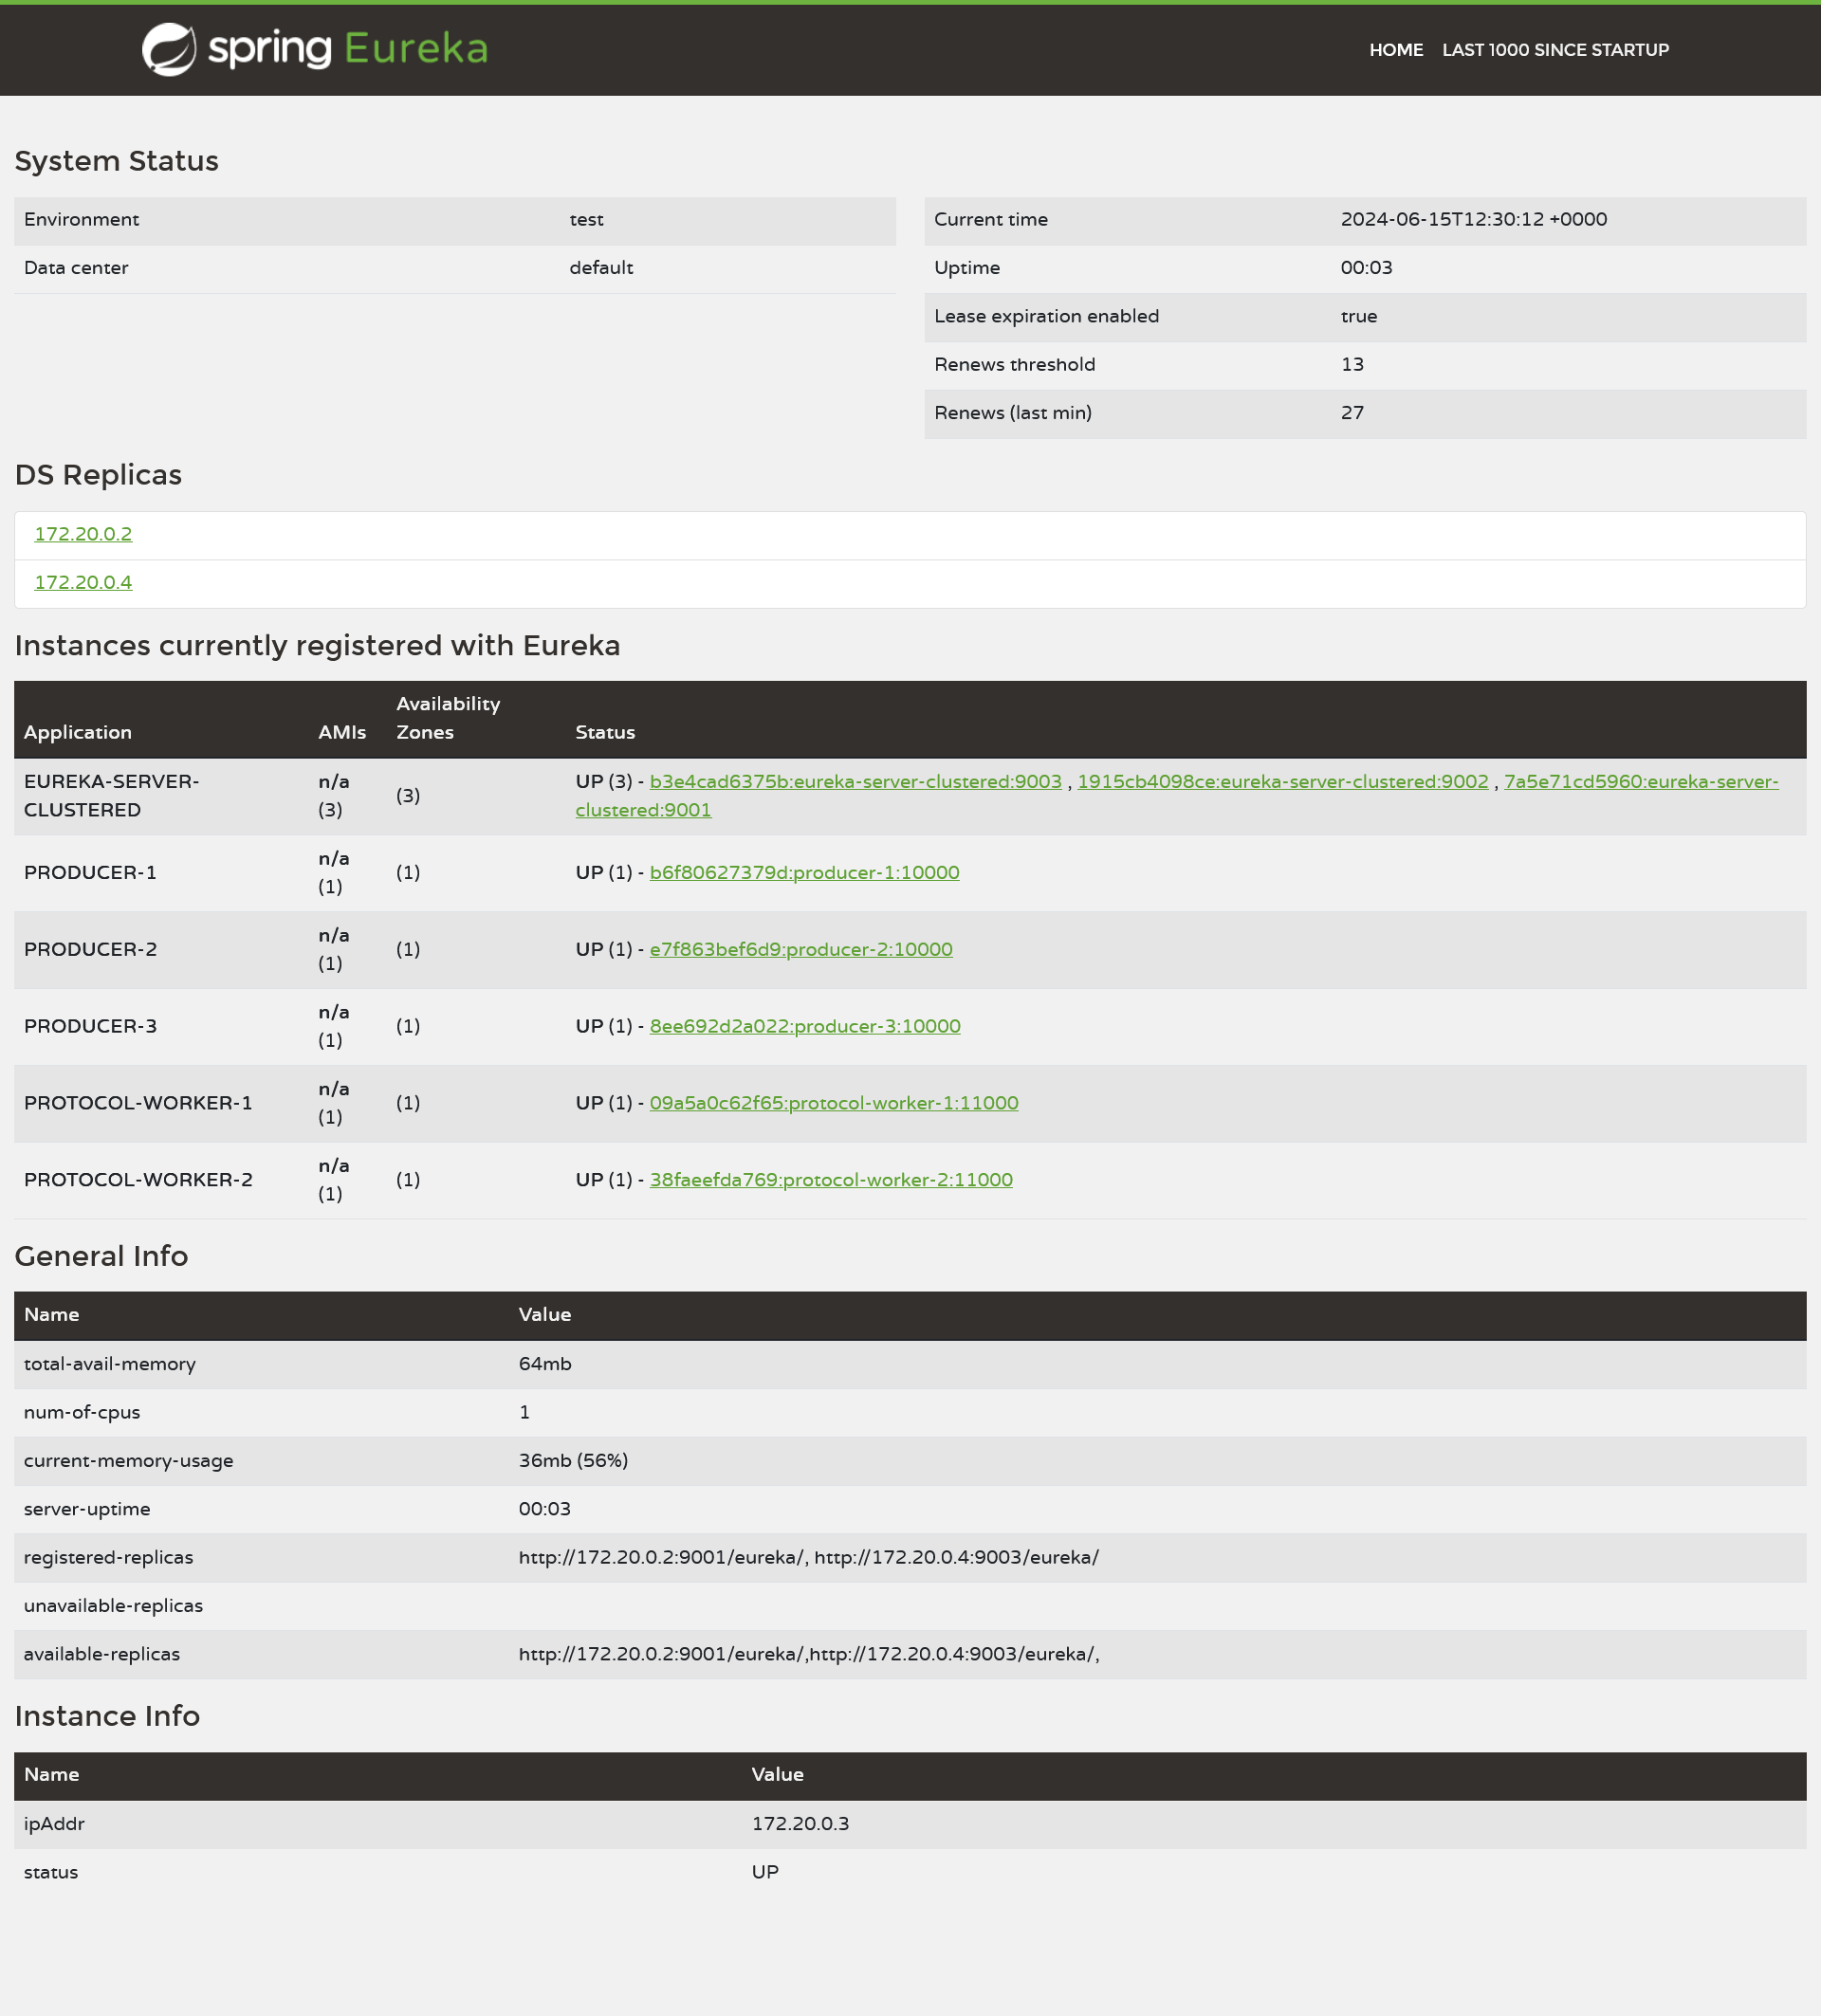
\includegraphics[width=\textwidth]{images/implementation/ServerDiscovery3Producer2Workers.png}
    \caption{Rejestr usług Eureka}
    \label{eurekaServerItems}
\end{figure}

Każda uruchomiona usługa typu producenta oraz węzła protokołu w podsystemie użytkowym jest rejestrowana w usłudze Eureka, gdzie aplikacja przechowywana jest pod unikatową nazwą, która jest wykorzystywana do odpytywania rejestru w usłudze klienckiej w celu otrzymania informacji o działających usługach w systemie. Rejestr przechowuje adresu pod którym usługa jest uruchomiona oraz jej stan. Na rys.\ref{eurekaServerItems} jest przedstawiony przykładowy stan usług zarejestrowanych w rejestrze Eureka.



\begin{lstlisting}[language=Java, caption=Implementacja rejestru usług serwera Eureka]
    
    package com.example.serviceregistry;
    
    import org.springframework.boot.SpringApplication;
    import org.springframework.boot.autoconfigure.SpringBootApplication;
    import org.springframework.cloud.netflix.eureka.server.EnableEurekaServer;
    
    
    @SpringBootApplication
    @EnableEurekaServer
    public class ServiceRegistryApplication {
    
    	public static void main(String[] args) {
    		SpringApplication.run(ServiceRegistryApplication.class, args);
    	}
    }
\end{lstlisting}

Kod usługi rejestru składa się z jednej klasy \verb|ServiceRegistryApplication| oraz metody \verb|main| uruchamiającej aplikacje. Jedyną linijką odróżniającą tę klasę od czystej aplikacji napisanej w frameworku Spring Boot jest adnotacja \verb|@EnableEurekaServer| odpowiada ona za uruchomienie usługi Eureka.

Głównym elementem określającym działanie usługi jest profil Spring Boot oraz wartości przypisane temu profiowi w pliku \verb|application.yml|. 

\subsubsection{Konfiguracja węzła rejestru}

Plik konfiguracyjny \verb|application.yml| jest plikiem YAML podzielony na trzy sekcje, każda opisująca oddzielny profil aplikacji oraz  pola konfiguracyjne niezbędne do prawidłowego działania klastra węzłów rejestru Eureka. 

\begin{lstlisting}[caption=Konfiguracja pierwszego węzła rejestru]
    spring:
      config:
        activate:
          on-profile: peer-1
      application:
        name: eureka-server-clustered
    server:
      port: 9001
    eureka:
      instance:
        preferIpAddress: true
        leaseRenewalIntervalInSeconds: 10
        leaseExpirationDurationInSeconds: 30
      client:
        registerWithEureka: true
        fetchRegistry: true
        serviceUrl:
          defaultZone: ${PEER_2_URL:http://localhost:9002/eureka/},${PEER_3_URL:http://localhost:9003/eureka/}
      server:
        enableSelfPreservation: true
        evictionIntervalTimerInMs: 1000
    logging:
      logstash:
        destinationOne: ${LOGSTASH_DESTINATION_ONE:localhost:5000}
        destinationTwo: ${LOGSTASH_DESTINATION_TWO:localhost:5001}
        destinationThree: ${LOGSTASH_DESTINATION_THREE:localhost:5002}
    
\end{lstlisting}

\subsubsection{Konfiguracja aplikacji}

Pole \verb|spring.config.activate.on-profile| określa, który profil aplikacyjny będzie aktywny podczas inicjalizacji usługi.

Pole \verb|spring.application.name| ustawia nazwę aplikacji na eureka-server-clustered. Nazwa ta jest wykorzystywana do identyfikacji oraz rejestracji aplikacji w klastrze Eureka.

Pole \verb|server.port| określa port urządzenia na którym aplikacja ma być uruchomiona.

\subsubsection{Konfiguracja instancji Eureka}

Pole \verb|eureka.instance.preferIpAddress| wartość tego pola ustawiona na \verb|true| określa preferowanie przez Eureka adresu \akronim{IP} (\english{Internet Protocol}) zamiast nazwy urządzenia do rejestrowania usług.

Pole \verb|eureka.instance.leaseRenewalIntervalInSeconds| ustawia interwał(w sekundach), co który instancja będzie wysyłać informacje o chęci odnowienia dzierżawy.

Pole \verb|eureka.instance.leaseExpirationDurationInSeconds| określa czas trwania(w sekundach), po którym instancja usługi zostanie uznana za wyłączoną, jeżeli aplikacja nie odnowi dzierżawy.

\subsubsection{Konfiguracja klienta Eureka}

Pole \verb|eureka.client.registerWithEureka| wskazuje, że instancja powinna zarejestrować się w serwerze Eureka.

Pole \verb|eureka.client.fetchRegistry| określa, czy ta instancja powinna pobrać informację z rejestru Eureka.

Pole \verb|eureka.client.serviceUrl.defaultZone| określa adresy \akronim{URL} (\english{Uniform Resource Locator}) usług równorzędnych serwerów Eureka w klastrze.

\subsubsection{Konfiguracja serwera Eureka}

Pole \verb|eureka.server.enableSelfPreservation| określa tryb samozachowawczy, który pomaga w utrzymaniu dostępności serwera Eureka nawet w przypadku partycji sieciowej lub dużych opóźnień.

Pole \verb|eureka.server.evictionIntervalTimerInMs| ustawia interwał (w milisekundach), dla którego ma być uruchamiane zadanie usuwania aplikacji których czas dzierżawy wygasł.

\subsubsection{Konfiguracja logowania zdarzeń}

Pola \verb|logging.logstash.destination*| ustawiają adres do usług zbierających dokumenty, do których będą wysyłane informacje o zdarzeniach w aplikacji producenta. Wykorzystuje zmienną środowiskową LOGSTASH\_DESTINATION\_*, która domyślnie jest ustawiona na localhost:5000, jeśli nie zostanie podana przy uruchomieniu aplikacji.\\[0.5cm]

plik \verb|application.yml| definiuje ustawienia konfiguracyjne dla aplikacji Spring Boot z różnymi profilami: peer-1, peer-2 i peer-3. Każdy profil konfiguruje aplikację jako część klastrowej konfiguracji serwera Eureka oraz wykorzystuje pozostałe uruchomione serwery Eureka jako repliki swojego rejestru w celu zapewnienia wysokiej dostępności w przypadku awarii jednego z węzłów w klastrze.

\subsection{Producent}

Producenci w systemach rozproszonych to komponenty lub usługi odpowiedzialne za generowanie i dostarczanie produktów lub danych. Służą jako źródło informacji lub towarów, które następnie są konsumowane przez inne części systemu. W przedstawianym systemie diagram klas usługi producenta został przedstawiony na rys\ref{ProducerUML}.

\begin{figure}[!htbp]
    \centering
    \includesvg[width=0.65\textwidth]{schemas/producer/Producer.drawio.svg}
    \caption{Producent - schemat UML}
    \label{ProducerUML}
\end{figure}

\subsubsection{Wymagania funkcjonalne}

Usługa producenta powinna spełniać następujące wymagania funkcjonalne:

\begin{itemize}
    \item Producent powinien sprawdzać czy dany produkt znajduje się w jego ofercie.
    \item Producent powinien sprawdzać czy ilość produktów zamawianych przez klienta jest możliwa przez niego do spełnienia. 
    \item Producent powinien zapewnić możliwość odbioru danych w celu sprawdzenia szybkości transmisji między nim a użytkownikiem.
\end{itemize}


\subsubsection{Główna klasa usługi producenta}

Główna klasa usługi producenta przedstawiona na rys\ref{producerMainClass}, jest podstawową klasą uruchamiającą aplikację z wykorzystaniem frameworku Spring Boot. Jest ona oznaczona adnotacją \verb|@EnableDiscoveryClient|, która zapewnia uruchomienie klienta Eureka w celu rejestracji w serwerze Eureka. Adres serwera na, którym aplikacja ma się zarejestrować  ładowany jest z konfiguracji aplikacji.

\begin{lstlisting}[caption=Główna klasa usługi producenta, label=producerMainClass]
    package com.example.producer;

    import org.springframework.boot.SpringApplication;
    import org.springframework.boot.autoconfigure.SpringBootApplication;
    import org.springframework.cloud.client.discovery.EnableDiscoveryClient;
    
    @SpringBootApplication
    @EnableDiscoveryClient
    public class ProducerApplication {
    
        public static void main(String[] args) {
            SpringApplication.run(ProducerApplication.class, args);
        }
    
    }
\end{lstlisting}

\subsubsection{Model produktu}

Klasa \verb|Product| przedstawiona na rys\ref{produktmodel} reprezentuje centralną jednostkę w ramach usługi Producenta.

\begin{lstlisting}[caption=Klasa reprezentująca produkt, label=produktmodel]
    package com.example.producer.model;
    
    import lombok.AllArgsConstructor;
    import lombok.Getter;
    import lombok.NoArgsConstructor;
    import lombok.Setter;
    
    @Getter
    @Setter
    @AllArgsConstructor
    @NoArgsConstructor
    public class Product {
        String id;
        String name;
        String model;
        String producer;
        Integer amount;
        Integer price;
    
        @Override
        public String toString(){
            return "[id = "+
                    id+
                    ", name=" +
                    name +
                    ", model=" +
                    model +
                    ", producer=" +
                    producer +
                    ", amount=" +
                    amount +
                    "price=" +
                    price +
                    "]";
        }
    
    }
\end{lstlisting}

Klasa ta jest opatrzona adnotacjami Lombok, \verb|@Getter|, \verb|@Setter|, które pozwalają automatycznie wygenerować funkcję dostępowe do zmiennych znajdujących się w klasie.

Klasa ta zawiera następujące zmienne:
\begin{itemize}
    \item \verb|String id| - Unikatowe dla danego typu produktu Id
    \item \verb|String name| - Nazwa produktu
    \item \verb|String model| - Model produktu
    \item \verb|String producer| - Nazwa producenta produktu
    \item \verb|Integer amount| - ilość produktu oferowana przez producenta
    \item \verb|Integer price| - cena produktu
\end{itemize}

Klasa ta zawiera też metodę \verb|toString()| która przeciąża domyślną metodę klasową języka java \verb|toString()| aby zapewnić reprezentację obiektu produktu, która zawiera wszystkie jego atrybuty.

\subsubsection{Serwis Produktów - ProductService}

Klasa \verb|ProductsService| zaprezentowana na listeningu\ref{productsServiceCode} jest usługą Spring odpowiedzialną za zarządzanie produktami w aplikacji producenta. Wykorzystuje ona klasę \verb|Product| w celu zainicjowania produktów, przechowywania produktów, oraz pobierania informacji o produktach. Klasa jest opatrzona adnotacją \verb|@Service|, wskazującej że jest to komponent usługi Spring, oraz \verb|@Slf4j|, aby umożliwić tworzenie dziennika zdarzeń w aplikacji.

\begin{lstlisting}[caption=Kod klasy ProductsService, label=productsServiceCode]
    package com.example.producer.service;

    import com.example.producer.model.Product;
    import com.fasterxml.jackson.core.type.TypeReference;
    import com.fasterxml.jackson.databind.ObjectMapper;
    import jakarta.annotation.PostConstruct;
    import lombok.extern.slf4j.Slf4j;
    import org.springframework.beans.factory.annotation.Value;
    import org.springframework.core.io.ClassPathResource;
    import org.springframework.stereotype.Service;
    
    import java.io.IOException;
    import java.io.InputStream;
    import java.util.ArrayList;
    import java.util.Collections;
    import java.util.List;
    import java.util.Optional;
    import java.util.stream.Collectors;
    
    @Service
    @Slf4j
    public class ProductsService {
    
        @Value("${products.file.name}")
        private String productFileName;
    
        @Value("${products.count}")
        private Integer count;
        private List<Product> products = new ArrayList<>();


        @PostConstruct
        public void loadProducts(){
            ObjectMapper objectMapper = new ObjectMapper();
            List<Product> tempProducts;
            try{
                ClassPathResource resource = new ClassPathResource(this.productFileName);
                InputStream in = resource.getInputStream();
                tempProducts = objectMapper.readValue(in, new TypeReference<List<Product>>(){} );
            }catch (IOException e) {
                log.error("Producer was unable to read products from file");
                throw new RuntimeException("Producer was unable to read products from file", e);
            }
            Collections.shuffle(tempProducts);
            this.products = tempProducts.stream().limit(this.count).collect(Collectors.toList());
        }

        public List<Product> getAllProducts() {
            return products;
        }

        public Optional<Product> getProductByName(Product product) {
            return products.stream().filter(listProduct ->  product.getId().equals(listProduct.getId())  && product.getAmount()<= listProduct.getAmount()).findAny();
        }
    }
\end{lstlisting}

Klasa \verb|ProductsService| zawiera następujące zmienne:
\begin{itemize}
    \item \verb|productFileName| - Nazwa pliku przechowującego produktu, z którego są ładowane dane przy starcie aplikacji. Wartość ta jest wstrzykiwana z konfiguracji aplikacji przy użyciu adnotacji \verb|@Value|.
    \item \verb|count| -  Liczba całkowita określająca liczbę produktów do załadowania. Ta wartość jest również wstrzykiwana z konfiguracji aplikacji.
    \item \verb|products| - Lista obiektów \verb|Product| zawierająca załadowane produkty.
\end{itemize}

Klasa \verb|ProductsService| zawiera następujące metody:
\begin{itemize}
    \item \verb|loadProducts| - Metoda opatrzona adnotacją \verb|@PostConstruct| zostaje wywołana automatycznie po inicjalizacji komponentu \verb|ProductsService|. Ładuje ona dane produktów z pliku znajdującego się w głównym folderze aplikacji. Następnie tablica jest mieszana w celu zapewnienia różnych produktów przy każdorazowym uruchomieniu aplikacji. Następnie tablica jest ograniczana do ilości produktów określonej w zmiennej \verb|count|.
    \item \verb|getAllProducts| - metoda zwracająca wszystkie produkty przechowywane w tablicy \verb|products|.
    \item \verb|getProductByName| - Metoda przyjmuje obiekt klasy \verb|Product| jako parametr i zwraca obiekt tej samej klasy opatrzony dodatkową klasą\verb|Optional<>|, który może służyć jako tymczasowy pojemnik z pustą wartość w momencie gdy szukany produkt nie zostanie znaleziony u producenta. W momencie wywołania funkcji tablica jest filtrowana w celu znalezienia czy produkt znajduje się w ofercie producenta oraz czy jego ilość spełnia szukane kryterium przesłane w obiekcie wejściowym.
\end{itemize}

\subsubsection{Kontroler prędkości transmisji - SpeedTestController}

Klasa \verb|speedTestController| przedstawiona na listeningu\ref{speedTestControllerCode} zapewnia punkt końcowy do testowania szybkości połączenia pomiędzy producentem a klientem poprzez odbieranie tablicy bajtów i zwracanie bieżącego czasu systemowego w nanosekundach. Punkt końcowy jest mapowany na \verb|/connectionSpeed| i obsługuję żądania \akronim{POST} protokołu \akronim{HTTP} (\english{Hypertext Transfer Protocol}).

\begin{lstlisting}[caption=Kod klasy SpeedTestController, label=speedTestControllerCode]
    package com.example.producer.controllers;

    import lombok.extern.slf4j.Slf4j;
    import org.springframework.http.ResponseEntity;
    import org.springframework.web.bind.annotation.PostMapping;
    import org.springframework.web.bind.annotation.RequestBody;
    import org.springframework.web.bind.annotation.RequestMapping;
    import org.springframework.web.bind.annotation.RestController;
    
    @Slf4j
    @RestController
    @RequestMapping("/connectionSpeed")
    public class SpeedTestController {
    
        @PostMapping
        public ResponseEntity<Long> testSpeed(@RequestBody byte[] data){
            log.info("Received connection speed request, size: {} bytes", data.length);
            return ResponseEntity.ok().body(System.nanoTime());
        }
    }
\end{lstlisting}

\subsubsection{Konfiguracja usługi producenta}

Plik konfiguracyjny przedstawiony na listeningu\ref{producerconfigFIle} służy do konfiguracji usługi producenta. Konfiguruje on właściwości aplikacji, ustawienia serwera, konfigurację klienta Eureka, konfigurację dziennika zdarzeń, szczegóły pliku produktów i punkty końcowe zarządzania.

\begin{lstlisting}[caption=Plik konfiguracyjny usługi producenta, label=producerconfigFIle]
    spring:
      application:
        name: producer-${PRODUCER_ID:producer-ERROR}
      servlet:
        multipart:
          max-file-size: 200MB
          max-request-size: 200MB
    
    server:
      port: ${PORT:10000}
      tomcat:
        max-swallow-size: 209715200
        max-http-form-post-size: 209715200
    
    eureka:
      client:
        service-url:
          defaultZone: ${PEER_1_URL:http://localhost:8761/eureka}
        register-with-eureka: true
        fetch-registry: true
    logging:
      logstash:
        destinationOne: ${LOGSTASH_DESTINATION_ONE:localhost:5000}
        destinationTwo: ${LOGSTASH_DESTINATION_TWO:localhost:5001}
        destinationThree: ${LOGSTASH_DESTINATION_THREE:localhost:5002}
    
    #name of products file
    products:
      file:
        name: "products.json"
      count: ${NUMBER_OF_PRODUCTS:1000}
    
    management:
      endpoints:
        web:
          exposure:
            include: "*"
\end{lstlisting}

\subsubsection{Konfiguracja aplikacji}

Pole \verb|spring.application.name| ustawia nazwę aplikacji. Wykorzystuje zmienną środowiskową PRODUCER\_ID, który domyślnie ma wartość "producer-ERROR", jeżeli zmienna środowiskowa nie zostanie podana przy uruchomieniu.

Pole \verb|spring.servlet.multipart.max-file-size| - konfiguruje maksymalny rozmiar pliku dla przesyłania plików wieloczęściowych do 200 MB.

Pole \verb|spring.servlet.multipart.max-request-size| - konfiguruje maksymalny rozmiar żądania dla przesyłania plików wieloczęściowych do 200 MB.

\subsubsection{Konfiguracja serwera aplikacji}

Pole \verb|server.port| ustawia port serwera. Wykorzystuje zmienną środowiskową PORT, która domyślnie wynosi 10000, jeśli nie zostanie podana przy uruchomieniu.

Pole \verb|server.tomcat.max-swallow-size| konfiguruje maksymalny rozmiar odbioru plików dla Tomcat do 200 MB.

Pole \verb|server.tomcat.max-http-form-post-size| konfiguruje maksymalny rozmiar żądania \akronim{POST} formularza \akronim{HTTP} dla serwera Tomcat do 200 MB.

\subsubsection{Konfiguracja logowania zdarzeń}

Pola \verb|logging.logstash.destination*| ustawiają adres do usług zbierających dokumenty, do których będą wysyłane informacje o zdarzeniach w aplikacji producenta. Wykorzystuje zmienną środowiskową LOGSTASH\_DESTINATION\_*, która domyślnie jest ustawiona na localhost:5000, jeśli nie zostanie podana przy uruchomieniu aplikacji.

\subsubsection{Konfiguracja pliku produktów}

Pole \verb|products.file.name| określa nazwę pliku przechowującego produkty.

Pole \verb|products.count| ustawia liczbę produktów którą producent ma świadczyć. Wykorzystuje zmienną środowiskową NUMBER\_OF\_PRODUCTS, która domyślnie wynosi 1000, jeśli nie zostanie podana.

\subsection{Węzeł protokołu}
\subsubsection{Podsystem monitoringu producentów}
\subsubsection{Podsystem propozycji zasobów}

\section{Uruchomienie środowiska}